\section{Model Description}
There two types of RW control torque interfaces, analog and digital. This modules assumes the RW is controlled through a set of voltages sent to the RW motors.  This module is developed in a general manner where a voltage deadband is assumed and the module can be run in a pure open-loop manner, or with a closed-loop torque tracking control mode.  Finally, if a RW availability message is present, then the RW is set to zero if the corresponding availability is set to {\tt UNAVAILABLE}. 



\begin{figure}[htb]
	\centerline{
		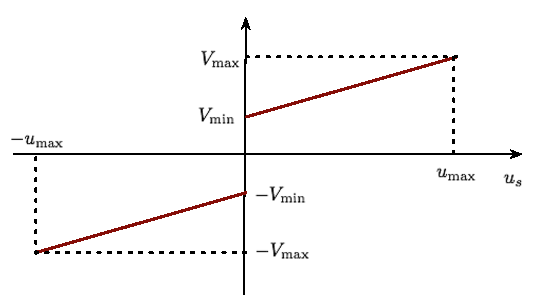
\includegraphics[]{Figures/us2V}
	}
	\caption{Illustration of RW motor torque to voltage conversion}
	\label{fig:us2V}
\end{figure}
\subsection{Open-loop voltage conversion}
This module requires the RW configuration message to contain the maximum RW motor torque values $u_{\text{max}}$.  The user must specify the minimum and maximum output voltages as shown in Figure~\ref{fig:us2V}.  The minimum voltage is a voltage below which the motor doesn't apply a torque, i.e. a deadzone.  

Let the intermediate voltage value $V_{\text{int}}$ as
\begin{equation}
\label{eq:rwMV:1}
V_{\text{int}} = \frac{V_{\text{max}} - V_{\text{min}}}{u_{\text{max}}} u_{s}
\end{equation}
The output voltage is thus determined through
\begin{equation}
V = V_{\text{int}} + V_{\text{min}} *\text{sgn}(V_{\text{int}} )
\end{equation}

\subsection{RW Availability} 
If the input message name {\tt rwAvailInMsg} is defined, then the RW availability message is read in. The voltage mapping is only performed if the individual RW availability setting is {\tt AVAILABLE}.  If it is {\tt UNAVAILABLE} then the output voltage is set to zero.


\subsection{Closed-loop commanded torque tracking}
The requested RW motor torque is given by $u_{s}$.  The RW wheel speed $\Omega$ is monitored to see if the actual torque being applied matches the commanded torque.  Let $J_{s}$ be the RW spin inertia about the RW spin axis $\hat{\bm g}_{s}$.   In the following development the motor torque equation is approximated as
\begin{equation}
u_{s} = J_{s} \dot\Omega
\end{equation}
where the assumption is made that the spacecraft angular accelerations are small compared to the RW angular accelerations.  The $\dot\Omega$ term is digitally evaluated using a backwards difference method:
\begin{equation}
\dot\Omega_{n} = \frac{\Omega_{n} - \Omega_{n-1}}{\Delta t}
\end{equation}
Care is taken that the old RW speed information $\Omega_{n-1}$ is not used unless a history of wheel speeds is available, in particular, after a module reset.  Thus, the actual RW torque is evaluated as
\begin{equation}
u_{n} = J_{s} \dot\Omega_{n}
\end{equation}
Finally, the closed loop motor torque value is computed with a proportional feedback component as
\begin{equation}
u_{s,CL} = u_{s} - K (u_{n} - u_{s})
\end{equation}
where $K>0$ is a positive feedback gain value.  Finally, this $u_{s,CL}$ is fed to the voltage conversion process in Eq.~\eqref{eq:rwMV:1}.  

\subsection{Saturation and Dead Band}
If the calculated voltage is outside of $\pm V_{\mathrm{max}}$, then the voltage is saturated at the $\pm V_{\mathrm{max}}$ value. Note, this corresponds to the reaction wheel torques being saturated. Similarly, if the calculated voltage is inside $\pm V_{\mathrm{min}}$, then the voltage is set to $\pm V_{\mathrm{min}}$. This simulates the dead band. If the $V_{\mathrm{min}} = 0$, then there is no dead band.